%!TEX root=report.tex
\subsubsection{Impulse responses}

The room impulse responses were computed for all positions following the procedure described in § \ref{sec:analysis}. The same assumptions on the speaker and microphones were made, however this time the echo created by the ceiling was considered as well.

The signal is quite noisy and the peaks are not easily discernible, but the primary echo, coming directly from the speaker, and the echo created by the ceiling are clearly visible in all responses. 
There is a small delay between the expected ceiling echo and the detected one which could be due to a imprecision in the latency measurement or because the speed of sound was not calibrated with the temperature.

Since the first steps of the robot were parallel to walls 1 and 3 and the last steps to walls 2 and 4 (see Figure \ref{fig:res3_room} for wall numbering), it would be expected that the peaks corresponding to those walls should remain constant while the other peaks should be moving according to the robot's movement. 
This phenomenon is not clearly discernible between positions 1 and 2 as shown in Figures \ref{fig:rir_1} and \ref{fig:rir_2}. It is more clear between positions 7 and 8, where the peak corresponding to wall 1 moves earlier in the signal as expected.

%An attempt was made to identify this movement using the cross-correlation between the two impulse responses at positions 7 and 8 (Figure \ref{fig:corr78}). Assuming that both responses are identical besides the two moving peaks, one would expect 2 peaks in the cross-correlation, corresponding to the time delay of the echoes induced by the robot's movement.
\begin{figure}
    \centering
    \begin{subfigure}{0.49\linewidth}
        \centering
        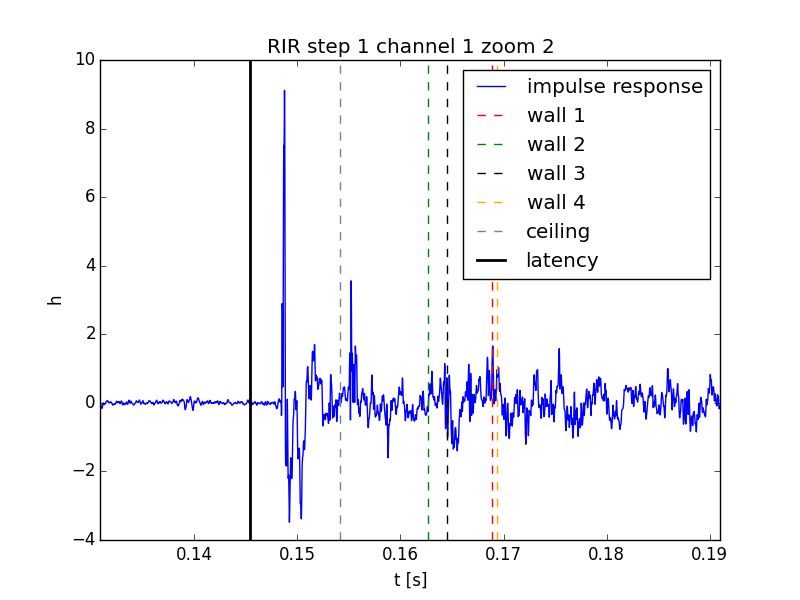
\includegraphics[width=\linewidth]{files/1_1_filt_zoom2.png}
        \caption{Position 1.}
        \label{fig:rir_1}
    \end{subfigure}
    \begin{subfigure}{0.49\linewidth}
        \centering
        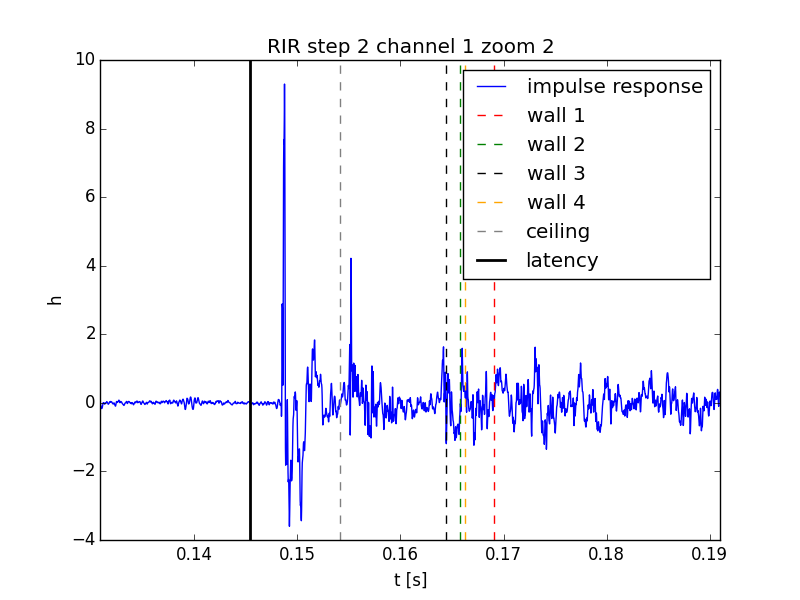
\includegraphics[width=\linewidth]{files/2_1_filt_zoom2.png}
        \caption{Position 2.}
        \label{fig:rir_2}
    \end{subfigure}
    \begin{subfigure}{0.49\linewidth}
        \centering
        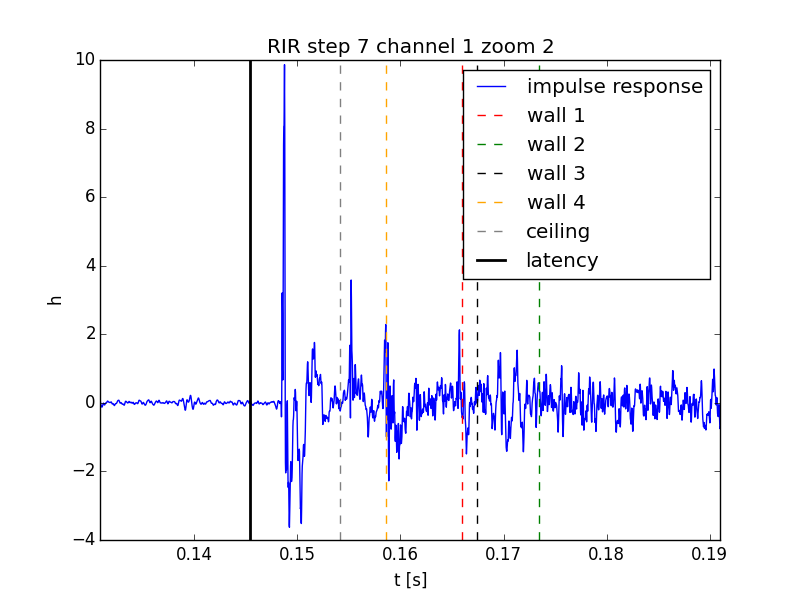
\includegraphics[width=\linewidth]{files/7_1_filt_zoom2.png}
        \caption{Position 7.}
        \label{fig:rir_7}
    \end{subfigure}
    \begin{subfigure}{0.49\linewidth}
        \centering
        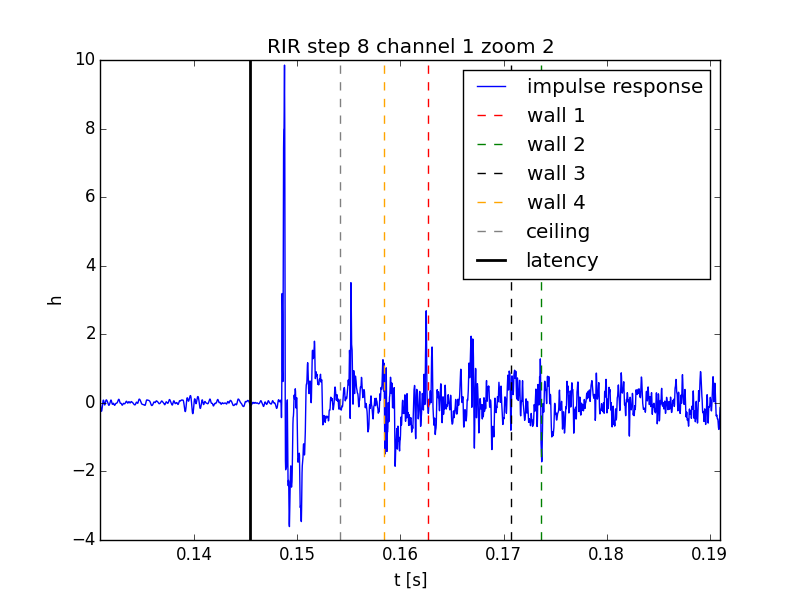
\includegraphics[width=\linewidth]{files/8_1_filt_zoom2.png}
        \caption{Position 8.}
        \label{fig:rir_8}
    \end{subfigure}
    \caption{Room impulse responses at Positions 1,2,7 and 8.}
    \label{fig:rir}
\end{figure}

%\begin{figure}
    %\centering
    %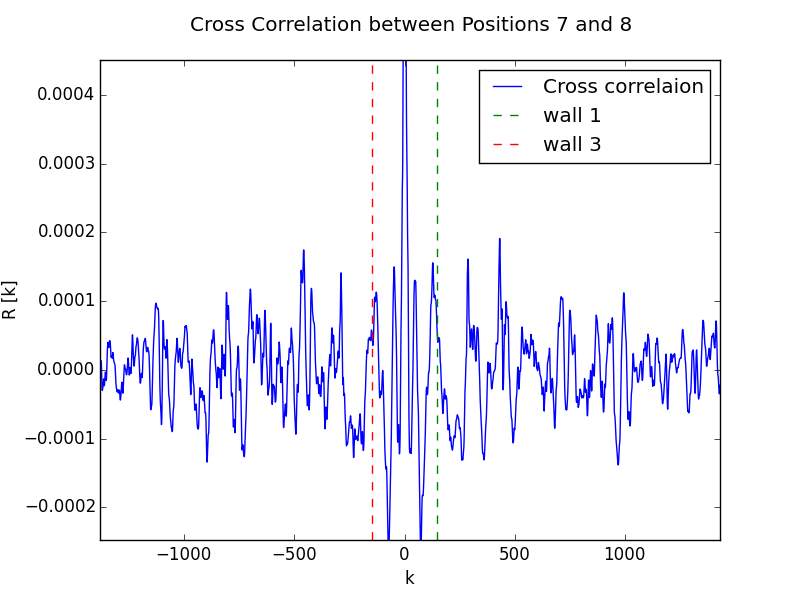
\includegraphics[width=0.6\linewidth]{files/CrossCorr78}
    %\caption{Cross-correlation between positions 7 and 8.} 
    %\label{fig:corr78}}
%\end{figure}

